\documentclass[12pt,addpoints,answers]{exam}
\usepackage[utf8]{inputenc}
\usepackage{amsmath,amsfonts,amssymb,amsthm}
\usepackage[margin=1in]{geometry}
\usepackage{mathtools}
\usepackage{hyperref}
\usepackage{fullpage}
\usepackage{microtype}
\usepackage{xspace}
\usepackage[svgnames]{xcolor}
\usepackage[sc]{mathpazo}
\usepackage{enumitem}
\usepackage{bm}
\usepackage{algorithm}
\usepackage{algpseudocode}

\pagestyle{head}

%----------Header--------------------%
\def\course{{\sc Fundamentos y Aplicaciones de Blockchains}}
\def\term{Depto. de Computaci\'{o}n, UBA, 2do. Cuatrimestre 2025}
\def\prof{Lecturer: Juan Garay}
\newcommand{\handout}[5]{
   \renewcommand{\thepage}{\arabic{page}}
   \begin{center}
   \framebox{
      \vbox{
    \hbox to 5.78in { \hfill \large{\course} \hfill }
    \vspace{2mm}
%    \hbox to 5.78in { \hfill \large{\prof} \hfill }
%       \vspace{2mm}
       \hbox to 5.78in { {\Large \hfill \textbf{#5}  \hfill} }
       \vspace{2mm}
       \hbox to 5.78in { \term \hfill \emph{#2}}
       \hbox to 5.78in { {#3 \hfill \emph{#4}}}
      }
   }
   \end{center}
   \vspace*{4mm}
}
\newcommand{\hw}[4]{\handout{#1}{#2}{#3}{#4}{Homework #1}}

% -- For ignoring stuff -- %
\newcommand{\ignore}[1]{}

\begin{document}

%----Specs: change accordingly-----%
\newif\ifstudent % comment out false
\studenttrue 
% \studentfalse

\def\hwnum{2}
\def\issuedate{25/9/25}
\def\duedate{14/10/25, 15:00 hs} % 
\def\yourname{Juan DElia} % put your name here
%------------------------------%

\ifstudent
\hw{\hwnum}{\issuedate}{Student: \yourname}{Due: \duedate}%
\else
\hw{\hwnum}{\issuedate}{\prof}{Due: \duedate}%
\fi

% \ignore{

\noindent \textbf{Instructions}

\begin{itemize}
    \item Upload your solution to Campus; make sure it's only one file, and clearly write your name on the first page. Name the file \textsf{`$<$your last name$>$\_HW1.pdf.'} 
    %{\bf Important:} Make sure to tap {\bf Turn in} after you upload your solution.   
      
     If you are proficient with \LaTeX, you may also typeset your submission and submit in PDF format. To do so, uncomment the ``\%\textbackslash begin\{solution\}'' and ``\%\textbackslash end\{solution\}'' lines and write your solution between those two command lines.
    
      \item Your solutions will be graded on \emph{correctness} and
    \emph{clarity}. You should only submit work that you believe to be
    correct.
    % , and you will get significantly more partial credit if you     clearly identify the gap(s) in your solution.
    
    \item You may collaborate with others on this problem set.  However,
    you must \textbf{{write up your own solutions}} and \textbf{{list
      your collaborators and any external sources (including ChatGPT and similar generative AI chatbots)}} for each
    problem. Be ready to explain your solutions orally to a member of the course staff
    if asked.
    
    \ignore{
    \item For problems that require you to provide an algorithm, you must
    give a precise description of the algorithm, together with a proof
    of correctness and an analysis of its running time. You may use
    algorithms from class as subroutines. You may also use any facts
    that we proved in class or from the book.
    } %IGNORE
    
\end{itemize}

\noindent This homework contains \numquestions\ questions,
% \numpages\ pages
for a total of \numpoints \ points.
% and \numbonuspoints\ bonus points.

%\medskip
\newpage

%} %IGNORE

\begin{questions}


\question We saw in class the notion of {\em digital signatures} and their security properties, {\em existential unforgeability} being an important one. 

\begin{parts}
    \part[5] Describe the purpose of a {\em Public-Key Infrastructure} (PKI). Can the security properties of a digital signature be guaranteed without a PKI? Elaborate.
    
    \begin{solution} %Uncomment and type your solution here
        El propósito de PKI es que haya una autoridad confiable, cuya public key es conocida, 
        mediante la cual podemos asociar a participantes de la red con sus correspondientes public keys.
        
        Las propiedades de seguridad de las firmas digitales no se pueden conseguir sin PKI:
        \begin{enumerate}
          \item Autenticación: Si no podemos asociar entidades con public keys no tenemos razon para creer
          que dicha entidad efectivamente firmo ese mensaje. Lo único que sabemos es que un mensaje fue enviado por
          quien posea dicha public key (que a priori es desconocido).

          \item Non-repudiation: La idea es que quien firmó, no pueda negar haberlo hecho. Si no hay una entidad que
          linkee a quien envió el mensaje y su public key, el recipiente del mismo no puede probar quien lo envió efectivamente
          (solo puede probar con que pk se firmó).

          \item Integridad: Esto si se mantiene, una vez firmado no se puede alterar al documento.

        \end{enumerate}
    \end{solution}

    \part[5] Bitcoin transactions use the ECDSA signature scheme. Does Bitcoin assume a PKI? If not, reconcile with the above argument.
 
    \begin{solution} %Uncomment and type your solution here
      Bitcoin no asume PKI. Esto no es un impedimento pues no es necesario vincular documentos y entidades reales, simplemente
      hay que asegurar que se guarden las transacciones entre nodos. Cuando se realiza una transacción quien la envía la firma con 
      su clave privada y quien la recibe puede verificarla usando la clave pública de quién la envió. (ahí es donde se usa el esquema de firmas).
      
      Estas transacciones luego son organizadas por los mineros que solo deberían aceptar transacciones validas. Recordemos que tenemos PoW
      para asegurar la inmutabilidad de los bloques.
    \end{solution}

\end{parts}

\newpage

\question[10] Refer to Algorithm 4 (Main Loop) in [GKL15]. We saw in class that blockchains would start from a ``genesis'' block, which would provide an unpredictable string to start mining from. Yet, notice that in Algorithm 4 mining starts from the empty string (${\cal C} \leftarrow \varepsilon$). How come? Explain why this works.

\begin{solution} %Uncomment and type your solution here
    El algoritmo inicialmente inicializa la cadena en si, podemos pensarlo como la estructura de datos, por eso es vacía al igual que st. 
    Inmediatamente después va a poner el flag init en falso y va a esperar a que aparezca una cadena para leer, y en caso de cumplir maxvalid() 
    mediante pow definir $C_{new}$ que puede ser la misma cadena o una que minó un bloque nuevo para finalmente broadcastearla.

    En el momento que se crea la blockchain entonces va a estar vacía. Alguien va a escribir el primer bloque (genesis) y mediante ese mecanismo
    va a ser difundida la nueva cadena que lo contenga, pues va a ser la más larga.

    Básicamente no se indica explícitamente el bloque génesis, pero mediante el algoritmo que va adoptando la cadena más larga, la 
    primer cadena que se adopte se debería seguir exteniendo. Así la primer cadena de longitud uno contiene al bloque genésis y de ahí
    en adelante se extiende sobre la misma.

\end{solution}

\newpage


\question Refer to Algorithm 1 ({\sf validate}) in [GKL15], which implements the {\em chain validation predicate}. 

\begin{parts}

\part[5] Rewrite {\sf validate} so that it starts checking from the {\em beginning} of the chain. 

% \begin{solution} %Uncomment and type your solution here

Asumi que existe la funcion tail que devuelve la cadena sin el primer elemento y first que dada
una cadena devuelve su primer elemento.

\begin{algorithm}
\caption{Validate chequeando desde el inicio de la cadena}
\begin{algorithmic}[1]
\Function{validate}{$C$}

  \State $b \gets V(\mathbf{x}_C)$
  \If{$b \land (C \ne \varepsilon)$}

    \Repeat

      \State $\langle s, x, ctr \rangle \gets \text{first}(C)$
      \State $s' \gets H(ctr, G(s, x))$
      \State $C \gets \text{tail}(C)$
      
      \If{$C = \varepsilon \land \text{validblock}_q^T (\langle s, x, ctr \rangle)$ } \Comment{Si es el ultimo solo chequea valid}
        \State break
      \EndIf

      \State $\langle s, x, ctr \rangle \gets \text{first}(C)$ \Comment{hay que chequear que el siguiente tiene su hash}


      \If{$\text{validblock}_q^T (\langle s, x, ctr \rangle) \land s == s'$}
        \State continue
      \Else
        \State $b \gets \text{False}$
      \EndIf

    \Until{$(C = \varepsilon) \lor (b = \text{False})$}

  \EndIf

  \State \Return $b$
\EndFunction
\end{algorithmic}
\end{algorithm}



% \end{solution}

\part[5] Discuss pros and cons of this approach, compared to Algorithm 1's.

\begin{solution}
  
  Este enfoque parece ser menos optimo que empezar desde el head. A priori pueden parecer igual de costos temporalemente 
  pero por la propiedad de common-prefix es preferible no empezar desde genesis.
  La mayor parte de los bloques del inicio son estables, donde en general podemos encontrar bloques que sean invalidos es al
  final de la cadena (los mas nuevos).
  
  Si vamos a rechazar alguna cadena empezar desde el genesis generalmente implicaria recorrela toda o casi toda porque los
  bloques invalidos suelen encontrarse al final. En cambio si empezamos por el final (bloques mas nuevos) vamos a encontrar
  esos bloques antes. 

  Basicamente este es un enfoque temporalemente menos deseable.
\end{solution}

\end{parts}

\newpage

\question {\bf Smart contract programming:} {\em Matching Pennies}. This assignment will focus on writing your own smart contract to implement the \href{https://en.wikipedia.org/wiki/Matching_pennies}{Matching Pennies} game. The contract should allow two players (A, B) to play a game of Matching Pennies at any point in time. Each player picks a value of two options---for example, the options might be \{0, 1\}, \{`a’, ‘b’\}, \{True, False\}, etc. If both players pick the same value, the first player wins; if players pick different values, the second player wins. The winner gets 0.1 ETH as reward. After a game ends, two different players should be able to use your contract to play a new game.

\noindent {\bf Example:} Let A, B be two players who play the game, each with 0.5 ETH.  A picks 0 and B picks 0, so A wins. After the game ends, A’s balance is 0.6 ETH (perhaps minus some gas fees, if necessary).

You should implement the smart contract and deploy it on the course's Sepolia Testnet.  Your contract should be as {\em secure}, {\em gas efficient}, and {\em fair} as possible. After deploying your contract, you should engage with other student's contract and play a game on his/her contract. Before you engage with a fellow student’s smart contract, you should evaluate their code and analyze its features in terms of security and fairness (refer to Lecture 10). You should provide:

\begin{parts}

\part[10] The code of your contract, together with a detailed description of the high-level decisions you made for the design of your contract,
including:  
\begin{itemize}
\item Who pays for the reward of the winner?
\item How is the reward sent to the winner?
\item How is it guaranteed that a player cannot cheat?
\item What data type/structure did you use for the pick options and why?
\end{itemize}

\begin{solution} %Uncomment and type your solution here

Dejo copiado mi contrato abajo de todo. 
Tambien se puede ver en 
\href{https://github.com/juandelia03/UBA/blob/main/Blockchain/HW2/matching_pennies/contracts/MatchingPennies.sol}{este repositorio}
donde tambien inclui los casos de test que verifican su funcionalidad basica. 
(Si se quiere correr en el directorio matching\_pennies hay que hacer npm i y despues npx hardhat test)


\begin{itemize}
\item Who pays for the reward of the winner?: 

Los jugadores le transfieren al contrato el eth necesario al momento de hacer el guess (manando el hash), una vez que que ambos
jugadores revelan su eleccion se actualiza en el mapping de jugadores el balance correspondiente sumandole 0.2 eth al ganador.
(0.1 que transfirio para jugar y los 0.1 que le gano a su rival). Asi que quien efectivamente paga al ganador es el contrato, 
usando los fondos ingresados por ambos, mediante withdraw.

\item How is the reward sent to the winner?:

La recompensa se envia al ganador mediante una funcion withdraw que usa transfer para enviarle los eth a quien la invoque. 
Esto es un esquema "pull", en lugar de transferirle al ganador su recompensa cuando gana el puede retirarla cuando quiera.

\item How is it guaranteed that a player cannot cheat?:

Un jugador no puede hacer trampa porque no se guarda directamente la eleccion de cada uno. En su lugar cada jugador envia un hash
al invocar guess() formado por un "secreto" que solo conoce cada uno y su eleccion. Una vez que ambos hicieron su guess se habilita
la funcion reveal, donde cada jugador puede efectivamente revelar que numero habia elegido mostrando su secreto y eleccion. Al
calcularse ese hash se compara con el ingresado originalmente como prueba de que esa fue su eleccion, aca se aprovechan
las propiedades de la funcion de hash.
Ademas no se permiten cosas como hacer 2 guess distintos, o cambiar el guess antes de revelar.
Otro detalle (no necesariamente trampa pero impide al gandor recibir su recompensa): Si un jugador revela su eleccion 
el otro podria decidir no revelarla para que no reciba su recompensa (a pesar de no verse beneficiado por eso), para 
remediar esta situacion hay una "deadline". Si a las 25 horas de juego un jugador no revela su eleccion y el otro si lo hizo, 
el ganador puede resetear el juego y asi obtener la victoria.

\item What data type/structure did you use for the pick options and why?:

La eleccion se guarda en un campo de un struct que representa a un jugador y que se mapea a su clave en un mapping. 
El tipo de dato que elegi en particular para choice fue bool porque solo hay dos opciones asi que no es necesario mas de un bit.
Como permitimos tener muchos jugadores y los guardamos a todos es una buena idea usar el dato mas chico posible para ahorrar espacio (gas).


\end{itemize}
\end{solution}

\part[5] A detailed gas consumption evaluation of your implementation, including: 
\begin{itemize}
\item The cost of deploying and interacting with your contract.
\item Whether your contract is {\em fair} to both players, including whether one player has to
pay more gas than the other and why.
\item Techniques to make your contract more cost efficient and/or fair.
\end{itemize}

\begin{solution} %Uncomment and type your solution here
  Direccion del contrato que deployee y donde hice las transacciones: 0x8b520161Bc8F1afA1d978BBdbfBe9B20B95eC7A4
  Para desplegar el contrato se uso 1,591,279 gas tx: 
  
  0x8eaddb2abb71825b4345876ae9b701860858f81c9962c4dfb3711b79ed913d5f.

  Se ve que el costo de hacer withdraw es el menos significativo de todos (28,780 gas). 
  Simplemente reescribe el balance de quien la invoca.


  Los join, la primera vez de cada jugador, tienen los mayores costos de gas porque deben agregar su struct al mapping. Costaron 66,508
  y 93,942 de Gas respectivamente. El segundo join consume gas extra porque hace lo mismo que el primero y finalmente setea la
  deadline.  

  Guess y Reveal tiene un costo similar pero hay una particularidad. Guess siempre realiza las misma operaciones, actualizan
  el flag guessed y el hash que se va a guardar en el struct correspondiente. Por eso los llamados de ambos jugadores van
  a tener siempre el mismo consumo de gas (52,396 gas). En cambio con reveal cuando el primer jugador la ejecuta solo se actualiza el
  flag revealed de ese jugador y se marca su eleccion (un boolean), por eso esa operacion cuesta incluso menos que el guess que
  escribe un bytes32. Pero cuando el segundo jugador hace reveal, ademas de hacer lo que hace el primero, actualiza el balance
  del ganador y resetea todas las variables para dar inicio a un juego nuevo. Es por eso que ese llamado resulta algo mas caro.
  Los costos son 37,497 gas y 63,132 gas respectivamente.

  Por las implementaciones de reveal y join el contrato no es del todo justo. El jugador que revele la segunda vez usa mas gas gas que el primero 
  y el jugador que se une segundo usa mas gas que el que se une primer 

  La otra diferencia en consumo de gas es la del ganador. Como el es el responsable de retirar los fondos va a pagar un
  costo extra. Igualmente esto pareceria lo justo porque alguien debe pagar esa fee para que el reciba los fondos. Si esto 
  no fuera asi  (por ejemplo en un esquema de push) quiza el otro jugador pagaria la fee para que el primero reciba su pago,
  lo que no pareceria del todo justo. 

  Para maximizar la eficiencia basicamente use pull y trate de usar la menor cantidad de memoria posible. Si hubiera usado 
  push cada vez que terminaba un juego se hubiera gastado una fee, aca un jugador puede jugar muchas veces y hacer un unico withdraw
      

  Las transacciones a las que me refiero estan en el inciso e) o en \href{https://sepolia.etherscan.io/address/0x8b520161bc8f1afa1d978bbdbfbe9b20b95ec7a4}{sepolia etherscan}

\end{solution}

\part[5] A thorough list of potential hazards and vulnerabilities that {\em may} occur in your contract; provide a detailed analysis of the security mechanisms you use to mitigate such hazards.

\begin{solution} %Uncomment and type your solution here
  A medida que iba desarrollando el contrato me tope con varias posibles vulnerabilidades que fui mitigando.

  \begin{itemize}
    \item Denial of service:

    El contrato debe permitir que dos jugadores jueguen a Matching Pennies y que una vez que terminen otra
    partida pueda empezar. Si simplemente iniciamos una partida y esta termina cuando ambos revelan su choice estamos ante un 
    escenario de DoS. Si alguno de los dos jugadores decide nunca revelar o hacer su guess el contrato queda inutilizado, nadie
    va a poder jugar hasta que esa partida termine. (Quiza el jugador que revela segundo ve que perdio y decide no revelar nunca).


    Para solventar esto defini una variable deadline que en el momento que el segundo jugador se une le pone un tiempo limite
    al juego. Si el juego no termino para ese momento cualquier persona puede interactuar con el contrato corriendo restartGame.
    
    Esta funcion hace lo siguiente: 
    
    1. Si ambos jugadores hicieron guess pero uno decidio no hacer su reveal, al reiniciar
    el juego se da como ganador a quien revelo su eleccion y recibe los fondos.  


    2. Si uno hizo guess y el otro nunca hace su guess, al reiniciar el jugador que hizo el guess recupera sus fondos.

    3. Si ambos jugadores deciden nunca hacer Guess no pasa nada.

    4. Si ambos jugadores hacen guess pero nunca revelan, no se les devuelven sus fondos a modo de penalizacion.

    Finalmente siempre reinicia el juego, permitiendo que nuevos jugadores puedan entrar a jugar.


    \item Front Running
    
    Por la naturaleza del juego hay que registrar de alguna manera que valor eligio cada jugador, pero guardarla
    directamente el el estado del contrato implicaria front running. Si guardaramos la eleccion de el primer jugador
    el segundo podria ver que eligio para ganar, pues la blockchain es publica.

    Para solventarlo implementamos un esquema para dar una prueba criptografica con la que un jugador pueda demostrar
    cual fue su eleccion inicialmente. Asi los jugadores no pueden conocer la de su adversario de antemano ni cambiarla.

    \item Reentrancy

    Dependiendo como implemtaramos el momento de transferir fondos podriamos tener problemas de reentrancy.
    Mi enfoque fue utilizar la funcion transfer, un esquema de pull y actualizar el balance interno del contrato antes 
    de transferir, cosa que si un atacante reentrara no cumpla las condicions para transferirle fondos.


  \end{itemize}

\end{solution}

\part[5] A description of your analysis of your fellow student’s contract (along with relative code snippets of their contract, where needed for readability), including: 
\begin{itemize}
\item Any vulnerabilities discovered?
\item How could a player exploit these vulnerabilities to win the game?
\end{itemize}

\begin{solution} %Uncomment and type your solution here
    Voy a hablar del contrato de Bruno Tievoli.

    En el contrato cuando un jugador se une tiene que hacer su commitment. Esta estrategia sirve para ahorrarle al jugador
    el costo de hacer una transaccion extra. El commitment es un hash, no se guarda explícitamente la choice sino una prueba
    de lo que eligio. 


    Los jugadores deben despues revelar su choice mediante la funcion reveal. Cuando el segundo jugador la ejecuta tambien
    se determina el ganador enviandole los fondos a quien corresponda y reiniciando el juego.

    Ademas se implemento un revealDeadline para prevenir denial of service. Si despues de 2 minutos los jugadores no terminaron
    se puede resetear el juego.

    Usa un esquema pull para retirar los fondos.

    En la funcion withdraw usa call para enviar los fondos asi que si bien teoricamente podria haber reentrancy, no
    serviria de nada porque antes de transferir se setea en 0 el balance del jugador.

    Pareceria no haber ninguna vulnerabilidad para explotar.
    
\end{solution}

\part[5] The transaction history of an execution of a game on your contract.

\begin{solution} 
    \href{https://sepolia.etherscan.io/address/0x8b520161bc8f1afa1d978bbdbfbe9b20b95ec7a4}{Ejecucion de un juego} 
    (captura de pantalla abajo)

    El flujo del juego es el siguiente:
    \begin{enumerate}
      \item Se une el jugador 1
      \item Se une el jugador 2
      \item Adivina 1
      \item Adivina 2
      \item Revela 1
      \item Revela 2
      \item El jugador 1, ganador, retira los fondos(opcional)
    \end{enumerate}

    Transaccion donde Jugador 1 recibe los fondos:

    0x7fe12933969055da7959add1428e4ab59b85608195236c881157ba1540774320

\end{solution}


    \begin{figure}[h]
        \centering
        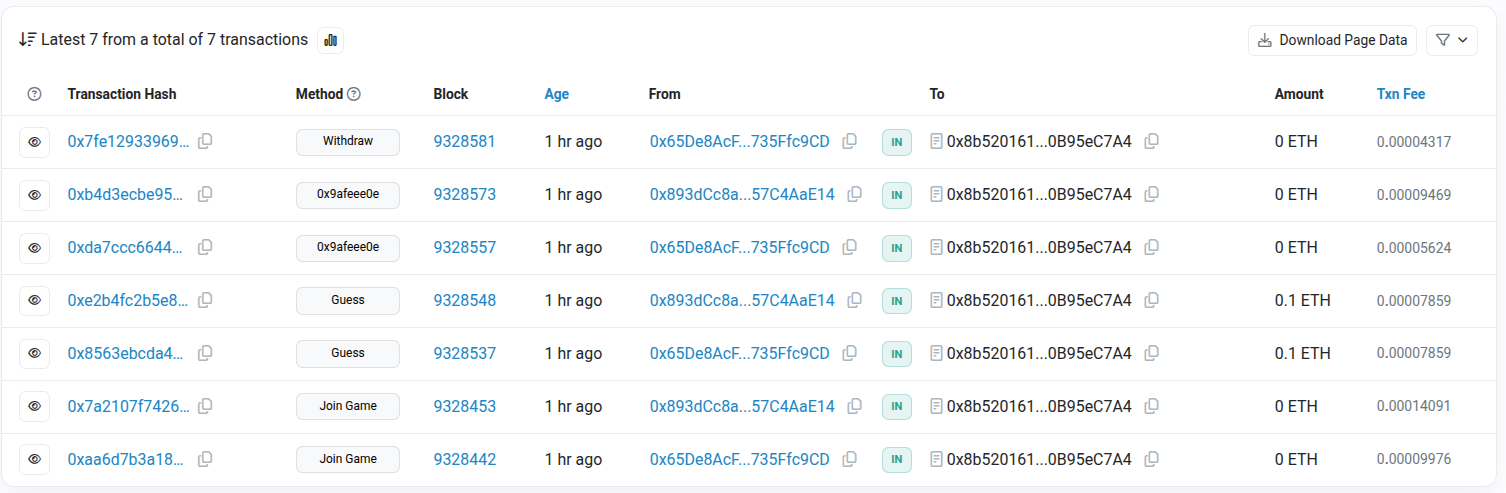
\includegraphics [width=0.8 \textwidth]{txs.png}
        \caption{Transacciones}
    \end{figure}  

\newpage

\begin{verbatim}

// SPDX-License-Identifier: UNLICENSED
pragma solidity ^0.8.28;

contract MatchingPennies {
    struct Player {
        bool present; // si hago playersMapping[add] con una address que no esta, present sera 0
        bool guessed;
        bool revealed;
        bool choice;
        bytes32 secret;
        uint256 balance; //balance que tiene para hacer withdraw
    }

    bool player1Ready;
    bool player2Ready;

    address player1Address;
    address player2Address;

    // si pasa cierto tiempo cualquiera puede resetear el juego
    uint256 public deadline;

    mapping(address => Player) public playersMapping;

    function updateSecret(address player, bytes32 _secret) private {
        require(
            !playersMapping[player].guessed,
            "No podes adivinar dos veces!"
        );
        playersMapping[player].secret = _secret;
        playersMapping[player].guessed = true;
    }

    function updateBalance(address player) private {
        playersMapping[player].balance += 0.2 ether;
    }

    function guess(bytes32 secret) public payable {
        require(
            playersMapping[msg.sender].present,
            "Solo pueden adivinar los jugadores de este juego"
        );
        require(msg.value == 0.1 ether, "Para jugar se debe enviar 0.1 ether");
        require(
            player1Ready && player2Ready,
            "Ambos jugadores deben estar listos para empezar a jugar"
        );

        updateSecret(msg.sender, secret);
    }

    function resetPlayer(address _playerAddress) private {
        playersMapping[_playerAddress].present = false;
        playersMapping[_playerAddress].guessed = false;
        playersMapping[_playerAddress].revealed = false;
        playersMapping[_playerAddress].choice = false;
        playersMapping[_playerAddress].secret = 0;
    }

    function revealSecret(bool _choice, bytes32 secret) public {
        // require(_choice == 1 || _choice == 0, "solo se puede elegir cero o uno");
        require(
            playersMapping[msg.sender].present,
            "Solo puede revelar su eleccion un jugador del juego"
        );
        require(
            playersMapping[msg.sender].secret ==
                keccak256(abi.encodePacked(_choice, secret)),
            "El secreto y choice deben ser los ingresados originalmente"
        );

        playersMapping[msg.sender].revealed = true;
        playersMapping[msg.sender].choice = _choice;

        //si ambos ya revelaron puedo actualizar el balance del ganador
        if (
            playersMapping[player1Address].revealed &&
            playersMapping[player2Address].revealed
        ) {
            bool choice1 = playersMapping[player1Address].choice;
            bool choice2 = playersMapping[player2Address].choice;
            if (choice1 == choice2) {
                updateBalance(player1Address);
            } else {
                updateBalance(player2Address);
            }
            //resetear a los jugadores y "desconectarlos" del juego
            resetPlayer(player1Address);
            resetPlayer(player2Address);
            player1Ready = false;
            player2Ready = false;
        }
    }

    function withdraw() public {
        require(
            playersMapping[msg.sender].balance > 0,
            "El balance debe ser mayor a cero"
        );

        uint256 balance = playersMapping[msg.sender].balance;
        playersMapping[msg.sender].balance = 0;
        payable(msg.sender).transfer(balance);
    }

    function joinGame() public {
        require(!player1Ready || !player2Ready, "Ya hay dos jugadores");

        if (!player1Ready) {
            player1Address = msg.sender;
            playersMapping[player1Address].present = true;
            player1Ready = true;
        } else if (!player2Ready) {
            player2Address = msg.sender;
            playersMapping[player2Address].present = true;
            player2Ready = true;
            //cuando se une el segundo jugador pongo un deadline
            deadline = block.timestamp + 24 hours;
        }
    }
    //para evitar
    // 1. Que un jugador no deje que juegue nadie
    // 2. que cuando un jugador revele el otro no lo haga porque sabe que perdio
    function restartGame() public {
        require(block.timestamp > deadline, "Deben pasar 24 horas");
        require(player1Ready && player2Ready, "No hay ningun juego en curso");
        //si algun jugador ya revelo y el otro hizo guess pero no revelo damos como ganador al que revelo
        if (playersMapping[player1Address].revealed) {
            // gana por abandono  1
            updateBalance(player1Address);
        } else if (playersMapping[player2Address].revealed) {
            // gana por abandono  2
            updateBalance(player2Address);
        }
        //si uno guessea y el otro no al pasarse el limite tiene la oportunidad de recuperar sus fondos
        else if (
            playersMapping[player1Address].guessed &&
            !playersMapping[player2Address].guessed
        ) {
            playersMapping[player1Address].balance += 0.1 ether;
        } else if (
            playersMapping[player2Address].guessed &&
            !playersMapping[player1Address].guessed
        ) {
            playersMapping[player2Address].balance += 0.1 ether;
        }

        //si ambos guessean pero ninguno revela o ninguno guessea el contrato se queda los fondos para penalizarlos

        resetPlayer(player1Address);
        resetPlayer(player2Address);
        player1Ready = false;
        player2Ready = false;
    }
}

\end{verbatim}

\end{parts}

\newpage

~\\

\end{questions}

\end{document}
